\documentclass{article}
\usepackage{graphicx}
\usepackage{float}   
\usepackage{verbatim}
\usepackage{amsmath} 
\usepackage{amssymb} 
\usepackage{fullpage}
\usepackage{listings}
\usepackage{subfig}   
\usepackage{epsfig}
\usepackage{siunitx}
\newcommand{\quotes}[1]{``#1''}
\usepackage{times}
\begin{document}

\title{MEAM520 Final Project Report}
\author{Brian Grimaldi, Venkata Gurrala, Sheil Sarda, Alexis Ward}
\date{December 14, 2020}


\maketitle


\section{Introduction}
    %Objective/Strategies (High Level)
    %Rules that were integral to our strategy
    %Point System (Equation)
In this final lab, we were tasked with using the skills we learnt throughout the semester to control the lynx robot in a head to head competition. This competition would test the teams' ability to navigate and pick up blocks from different platforms to drop them in the goal platform. Bonus points are given for being able to manipulate the orientation of the blocks such that the white face of the block is facing upwards as well as being able to pick up and drop dynamic blocks. These dynamic blocks are placed in between the two opponents on a turn table. The static blocks are only reachable within each team's robot. The blocks are randomly placed on the map to prevent any hardcoded movements to score points. The points are assigned according to the following formula where the altitude of the block can be manipulated by stacking blocks:
\[
points=value*(1+\frac{altitude}{10}+sidebonus)
\]

The general strategy used was to get as many dynamic and static blocks to the goal as possible. In particular, the dynamic blocks were prioritized first due to the fact that it had 3 times the number of points and were open to be taken by the other team. The dynamic blocks were stacked in a specific part of the goal position. To avoid the risk of a falling stack, the stacks for dynamic and static blocks were positioned apart at the goal platform. All the blocks in the work space can be picked up from a vertical or horizontal wrist orientation. While picking up the dynamic blocks, the horizontal wrist position was used so that we could enable a larger tolerance to grasp a block. Additionally, by using a horizontal wrist orientation, we were able to push forward upon blocks so that the orientation of the blocks aligned with the orientation of the end effector. For static blocks, a vertical orientation to pick up blocks was prioritized. By enabling the use of the rotating wrist, the end effector could easily align with the orientation of the blocks. However, not all static blocks were able to be picked up from a vertical orientation due to the fact that some blocks lied on the edge of the reachable workspace and would cause a non-feasible orientation. In this scenario, a horizontal wrist orientation was used, similar to what was used for picking up dynamic blocks.

\section{Method}
    \subsection{Dynamic Blocks}
    %Sheil/Venkata
    When attempting to pick up dynamic blocks, a home position for the dynamic block picking was first defined. This is the location where the end effector is in close proximity to the rotating turn table where it is ready to position itself to approach a target block on the turn table. Figure \ref{dyn} shows a picture of this position. As soon as the robot reaches the home position, it calculates all of the current blocks' state and determines their current angles by using the x and y position components of the transformation matrix and using the atan2 function. The angles of each block are then checked and compared in order to find the block which has smallest angle to the end effector's angle of 45 degrees from the x axis. It prioritizes the closest angle in the direction of the turntable movement. It then targets the closest block and positions the wrist such that it is 50 mm behind the block when the block is in the same plane as the robot’s wrist, as shown in figure \ref{dyn2}. Figure \ref{dyn2} indicates the method used to determine the configuration that would enable the robot to wait 50 mm behind a given block. Using the transformation matrix of the block, the variable r can be found which is the distance between the block's center and the turn table's center. The constant A is known since it is given that the offset of the robot's base is 200 in the x and y direction. The offset is the shortest distance between the robot's base and the desired end effector's position which is 50 mm behind the block. This offset is used to then determine the x and y positions of the end effector which can be plugged into the calculate IK function to return the robot's configuration. After this position is determined, the robot waits for the block to come closer to the angle that the arm is at. The block’s state is constantly tracked for any updated movement due to both the turn table and movement caused by opponent. When the block’s angle is within 0.05 radians of the angle of the static wrist, the robot is given the command to simply move forward in its plane. The command is given to move further forward than the block’s current position so that any difference in orientation can be fixed and the end effector can have a secure grip on the block. 
    \[
    r=\sqrt{x^2+y^2}
    \]
    \[
    A=\sqrt{2*200^2}=282.85 \\
    \]
    \[
    Offset=A-(r+50) \\
    \]
    \[
    x pos=y pos=\frac{Offset}{\sqrt{2}}\\
    \]
    
    \subsection{Static Blocks}
    %Venkata/Alexis
    To pick up each static block from the remaining platforms, we compute two desired homogeneous transformation matrices – one to approach the block ($T_b$), and one to grab it ($T_a$) – and then use inverse kinematics to get the necessary sets of joint values. $T_b$ and $T_a$ only differ in their last (position) columns. The distance between these positions and the current block is passed in from final.py (by default, 50mm and 10mm, respectively) We use two main techniques to get these matrices. 
    
    The first, and most common, option is to approach the block from above if that is a feasible transformation within the robot’s reachable workspace. We start with a Rotation matrix that represents an end effector pointing downwards (assuming all other joint angles are 0), we post-multiply it by a Z-Rotation matrix computed from Joint 4’s current value, and then we pre-multiply it based on the value Joint 1 needs to have for the robot to point at the block. Paired with the block’s location, this functionally positions the robot right at the block. However, we want to grab it as smoothly as possible, so we then find the shortest rotation that Joint 4 needs to make to align the end effector with the block’s pose. We rotate our matrix again by this new value, and we now have a rotation matrix that perfectly aligns the gripper’s axes to the cube axes. To increase our chances of a sideBonus, we also check if one of the gripper’s sides are touching the block’s white face, and, if so, we rotate the end effector again by 90 degrees. To create the final homogeneous transformation matrices, we use our Rotation matrix in the first three columns, and then use the block’s position shifted upwards (by 10 and 50mm) for the fourth. View calcNewQ4 under Implementation for more details.
    
    Otherwise, we approach the block from the side (with the last joint link and end effector parallel to the world X-Y plane). For this option, we do not care about the block’s initial orientation. Our approach matrix ($T_b$) begins close to the block, and the second grab matrix ($T_a$) positions the robot to push forward into the block’s space – 20mm ``closer’’ than the default - sliding the block to align its orientation close to that of the end effector, similar to the dynamic approach. We get the orientation of our transformation matrix through a simple cross product, knowing that our gripper’s desired Z-axis is the normalized vector from the robot origin to the block origin (flattened to the world X-Y plane), since we want the robot pointed at the block. View getSideMat under Implementation for more details.
    
    If neither of these two options are possible, there is a backup calculation to approach the block at an angle. we use the same calculation as above, except the Z-axis is instead the normalized vector from a desired Joint 2 location to the block. However, this has never been necessary. View the angled=True subsection getSideMat for more details.
    
    To decide between these three methods,  we do a quick computation to check to see if theoretical joint positions would be possible based on the robot’s link lengths and joint limits.
    
    The static section of final.py then uses these two matrices in the following order: q($T_b$) with the gripper at width 30, q($T_a$) with the gripper at width 30, q($T_a$) with the gripper at width 0, and then q($T_b$) with the gripper at width 0 to lift the block out of the way before positioning the it at the goal position as determined below.

    
    %need to talk more about grip static 
    \subsection{Goal Positioning/Stacking}
    %Alexis/Sheil
    
        With the objective of maximizing the altitude of all the blocks on our goal platform, we decided to implement block stacking. We considered several implementation options, including tracking the position of the blocks currently on the platform and using the pose of the top most block of the stack to determine where the robot arm should drop the block. A common shortfall of this method is that if due to mechanical error, the top block is not centered on the previous block, this error will propagate up the stack, causing instability and eventually lead to a toppling over.
		
		A simpler implementation we implemented in our robot was to generate a smooth path of moving the end effector to the $X, Y$ coordinate of the center of the stack, but maintaining an altitude greater than the largest possible height of our 3-block stack. From this position, we relax the end effector and drop the block onto the tower in a controlled purely vertical motion.
    
    \subsection{Path Planning}
    %Venkata
   The paths that the robot took throughout its run were developed to avoid collisions with the platform as well as the blocks. Since the blocks were randomized, there would be a chance where the static or the dynamic blocks could be stacked on top of each other for the run. If the robot was not handling with blocks on a given platform, it was completely out of the vertical space of the platform to prevent knocking over stacked blocks. Rather than using path planners, a hard coded path was developed which we determined would be more reliable since it is deterministic and would allow us to optimize for the shortest path required to move between platforms while considering the handling of the blocks between the platforms. After each dynamic block was picked up, it was taken to a preset position on the goal platform. There were 2 intermediate commands given in the path before it went into the goal platform space. The first was the zero position and the second was the position right before entering the goal platform from a vertical position. The second intermediate command was given so that the robot's theta 1() was constant so that the arm's swinging motion would not cause any present stacks on the platform to fall over. After the last dynamic block was placed in the goal position, the robot was then tasked to move pick up the static blocks at the platform closest to the goal position. This enabled the robot to quickly score as many points as possible, given the allotted time. After each static block was picked up, it slowly came out of the z axis space above the platforms before moving to the goal position to prevent any stacks on the goal from falling over. By using anywhere between 2 to 3 preset intermediate commands, we were able to eliminate the need to compute a path using a path planner such as a potential field or an RRT planner, thus saving valuable time. 
 
   
% Combine with Methods
% \section{Concepts utilized in Code}

%     \subsection{final.py}
    
    
%     \subsection{calcIK.py}
    
    
%     \subsection{gripStatic.py}


%     \subsection{Grasping}
%     %How we decide to grasp moving or static blocks.


\section{Experimental results}
%Draw upon results of the match
%Are cases chosen show advantages and disadvantages
%Brian
When our simulation is run with no time constriction, we find that our robot is able to successfully stack 5 dynamic blocks on top of one another and 2 static blocks in a second stack.  On the third static block, our robot knocks over the stacks due to an error in positioning for the second stack.  This scenario takes a couple of minutes to reach this conclusion.

In competition, our robot was able to perform and stack well in more ideal scenarios, but under performed in situations we did not account for.  In Figure \ref{data} we find our data results from across the four matches during the round robin.  We record the blocks that we pick up and whether they were dynamic or static.  We also record the time at which the block is picked up in the span of the 60 second match, the number of stacks, the height of the stack, and the time spent waiting for a dynamic block at the turntable in the center of the map.  

In our match with Team 6, we were able to pick up 1 dynamic block within 5 seconds as seen in Figure \ref{t6}.  However, our robot got stuck at the goal position, failing to release the block until about the 45 second mark.  Our robot was able to pick up a second block around the 50 second mark, but did not release the block in time to be counted.  As a result, we finished with one stack of one dynamic block.  

In our second match with Team 7, we were able to pick up 3 dynamic blocks as seen in Figure \ref{t7}.  In this match, our robot was able to consistently pick up the blocks, taking some time to wait for a dynamic block due to it choosing blocks that were further away on the turntable than other blocks.  Our robot was not impeded by Team 7's robot on the dynamic turntable since their robot focused entirely on static blocks.  As a result, our robot was able to score enough points to win, with a 1 stack of 3 dynamic blocks.

In our third match with Team 8, we were unable to pick up any blocks, as our robot was frozen at the dynamic turn table.  Team 8's strategy was to knock off all dynamic blocks on the turn table, leading no team to pick up blocks.  By making this assumption about the opposing teams strategy, they were able to impede teams that went to the turn table first.  By knocking all blocks off of the table before we were able to pick one up, they consequently froze our robot since it is looking for a block that is not currently in play.  As a result, our robot did not score any points due to not picking up any blocks.

In our final match with Team 9, we were able to pick up 4 blocks, 2 static and 2 dynamic as seen in Figure \ref{t9}.  In this match, we were competing with the opposing team for dynamic blocks.  Due to the slow nature of our dynamic pick up algorithm, we were able to pick up only 2 blocks, with the first one taking the longest to place down at the goal and the second being grabbed shortly after.  Due to the turn table being empty, our robot began acquiring static blocks from the platform closest to the goal.  Our robot was able to pick up the static blocks with some efficiency.  It was able to successfully stack 2 blocks, and picking up a third block but unable to place it on the stack.  However, as seen in the ideal scenario, if the motion were completed, it would knock over all of our successful stacks.

\section{Implementation}
% TODO
% Brief overview of the key functions in our code base
% - Description of func + inputs and outputs
% - pseudocde where necessary
% - where the fucntion is located (i.e. file name and line number)

\subsection{gripStatic.py}
    \subsubsection{calcNewQ4}

    Named as such because it originally only calculated q[4], this function finds the desired homogeneous transformation matrices to approach a block. It takes in inputs: q, the 1x6 vector of current joint inputs; pose, a 4x4 matrix defining the current block position and orientation; color, a string of either ``blue’’ or ``red’’; and a, a length 2 array determining the distance the robot should be from the block. It outputs two 4x4 desired T0es. $T_a$ being the transformation matrix that locate the robot at the block; $T_b$ positions the robot a distance away for the approach.
    
    This method declares different values for the varables cons, origin, startDir, and effectorDown based on color; it allow sfor this method to work for both the red and blue robots. Using \textbf{inRange}, we check if we can approach the robot from above. (If not, we use the method \textbf{inRange} to return $T_a$ and $T_b$).
    
    Starting with a basic Rotation Matrix pointing in the negative Z direction, we post-multiply it by a Z-Rotation matrix computed from Joint 4’s current value, q[4], and then we pre-multiply it based on the \textbf{angularDifference} between the vector startDir (where the robot points in its 0 state) and blockDir (the vector from the robot origin to the block).  We then find the shortest rotation needed to align this Rotation Matrix with the block’s pose, done in \textbf{ checkCubeAngle} below. We make sure to clamp this value to the joint limits (by offsetting it by 90 degrees if it exceeds the limits). We once again post-multiply our Rotation Matrix by a Z-Matrix based on this angle, getting our near-final gripper orientation. To increase our chances of a sideBonus, we also check whether one of the gripper’s sides is touching the block’s positive-z face by comparing the block’s z-axis with the gripper’s x-axis (using a dot product). If so, we rotate the end effector again by 90 degrees (once again bound by the joint limits). We return two homogeneous transformation matrices using this rotation matrix and position values above the block’s location (offset by a[0] and a[1] in the Z direction).
    
    \subsubsection{checkCubeAngle}
    This function gets the angle between a given frame and the world space rotation of a cube. It takes in inputs: cubeR, a 4x4 matrix defining the current cube position and orientation; rotAxis, [0, 1, or 2] defining the axis of rotation of the current frame, Z by default; and jointR, a 3x3 matrix defining the Frame to compare the block to. First, this function determines which cube axis points upwards (or downwards), then, knowing that the two other axes are flush to the world X-Y plane, we get the angularDifference between one of these axes and a non-axis-of-rotation for the reference frame. We mod this angle so that it is of magnitude 45 degrees at a maximum.
    
    \subsubsection{angularDifference}
    
    Gets the magnitude of the angle between two vectors using the law of cosines, and then gets the direction of rotation using a simplified cross product (based on the given axis of rotation).
    
    \subsubsection{getSideMat}
    
    Through this function, on input angled=False, we know that the gripper must be parallel to the X-Y plane, and thus the end effector’s Y-axis will be (0, 0, 1) in world space. The gripper’s desired Z-axis is given. Now, to get the X-axis, we just take the cross of the gripper’s Y and Z axes. These (x, y, z) vectors are the 0th, 1st, and 2nd columns of $T_a$ and $T_b$. The last position columns are the positions of the block offset (along this local Z-axis) by the distances passed in from final.py.
    
    On input angled=True, the Z-axis is not necessarily parallel to the X-Y plane. We follow the calculation from above, but we also recompute the Y-axis after the fact using the cross of the gripper’s X and Z axes.
    
    \subsubsection{horizontalAngle}
    
    An easier way to call getSideMat (calculates inputs z and cons on its own). This is used in final.py to place blocks at their goal positions.
    
    \subsubsection{inRange}
    For the robot to come from above, check to see if a point positioned  L4+L5 above the block (a theoretical joint 3) is within L2+L3 distance of joint 1 (L1 above the origin). For the robot to come from the side, compare the theoretical Joint 3 to an angled Joint 2. If neither of these positions are in the right range, we default to the “angled” method. This is just an approximation, and not as effective as checking the isPos value from an IK calculation, but it is much quicker.

\subsection{final.py}
    \verb|final.py| has 3 functions, setpath, closestblock and avail\_dyn.  Alongside these functions, this file also contains the necessary code to control our robot in a competition or testing environment.  
    
    \subsubsection{setpath}
    The setpath function has one parameter passed through and no output.  When setpath is called, a configuration is passed into it.  First, this function initializes a "ispos" flag, checking to see if the robot is at the desired position.  After this initialization, the function commands the robot arm to move to the desired position.  While ispos is false, we check to see if the difference between the current configuration and the desired configuration is within a certain threshold, which in this case is an error of 0.05.  It checks joints 1 through 5 for this error.  If all joints fall within this threshold, ispos is true and the function ends, returning nothing.
    
    \subsubsection{closestblock}
    The closestblock function takes in one parameter, color which distinguishes the color robot that we are currently using.  We first store the name pose and twist of the objects in the current map for future reference.  Next, we call the avail\_dyn function which returns all available dynamic blocks on the turn table.  With this list, we can then initialize and a block angle and angle difference array.  For the range of 0 to the length of available blocks, we determine the angle of our block currently on the turn table.  Depending on where the block is currently, we do a simple arctan calculation with or without the addition of $2\pi$.  After calculating the block angle, if the color is red or blue, we determine the angle difference between our robots end effector and the block angle.  Next, by using an argmin or argmax function, we can determine the index for the closest block to our end effector.  Once we determine this index, we return the index of the dynamic block to be used in other functions.  
    
    \subsubsection{avail\_dyn}
    The avail\_dyn function takes in no arguments., returning a list of dynamic blocks on the turn table.  Once we have checked the x, y and z bounds of the turntable for each block, we append that block to the empty list, subsequently populating our list with only blocks on the platform.  Finally, this list is returned to be used in another function.
    
    \subsubsection{Main Code}
    The main portion of our code is run on execution of our code.  First, it takes in the terminal argument for the color that we wish to control in the simulation (red or blue, subsequently assigning the desired colored lynx robot to the lynx parameter.  Before doing any calculations, we use the wait\_for\_start command to wait for the match to begin by the moderator.  When the match starts, we sort all dynamic blocks into one list and the static blocks for the desired colored robot into a second list.  With our blocks stored into our lists, we  then determine where the blocks are specifically in the map.  More specifically, we determine which platform the 8 static blocks are placed on by using a simple for-loop and conditional statements. 
    
    With all our blocks properly sorted, we begin to focus on collecting dynamic blocks per our determine game plan.  We found a set transformation matrix at which we wish to orient our lynx arm, where it is parallel with the dynamic turn table, perpendicular to the tangential line of the table relative to the current robotic arm.  We find the configuration of this position by utilizing our calcIK inverse function.  With this configuration, we move our robot and begin looking for the closestblock to the end effector.  With this index, we store our chosen block in a variable and set our end effector to be 50 mm away from the predicted position of the block.  Through mathematical calculation seen in Figure \ref{dyn_alg} on lines 168 through 186, we determine the current angle of the block at a given time.  Depending on our color of the robot, we begin to wait for the difference of the angle of the block and our robotic end effector to fall within a certain threshold, moving forward to grab the robot once it does.  Finally, the block is lifted towards the goal position, placing/stacking the block in a designated spot for the dynamic blocks.
    
    
    %Alexis could you check this?  Not entirely sure what is going on in this section with the two transformation matrices.
    Once there are no more dynamic blocks left on the turn table, we begin to pick up the static blocks on platforms 1 and 2.  Depending on the color of our robot, we determine a fixed goal position to drop/stack our static blocks at.  We utilize the calcNewQ function described earlier to generate a transformation matrix that will bring our robot to a given block on the platform, picking it up from the side or from above depending on what position is feasible given our robots limitations.  With the block grasped, we generate another set of transformation matrices using the horizontalAngle function that will bring our robot to the desired area for the static block stack  These transformation matrices determine how high up the robot needs to place the block in order to avoid knocking over any previous stack that was made.  
    
    
  
\section{Evaluation}
%Analyze the results of the match
%Brian(?)
%Blocks stacked in certain time
    %Static/Dynamics?

     \subsection{Stack Height}
	    As seen in Figure \ref{ideal}, we were able to successfully stack 5 dynamic blocks on top of one another without disturbing the stack in any way.  We chose not to stack higher than this height as error of stacked blocks might propagate upwards, causing the stack to fall.  However, as noted in both the ideal case and the match against team 9, the static blocks were only able to stack up to two blocks high.  We believe this is due to an inconsistency between our dynamic stacking method and static stacking method being developed separately.  As a result, this would lead to slightly different but generally similar algorithms.  This issue can be fixed simply by fine tuning the height at which the static blocks should be dropped.  This would avoid collision with the stack it is aiming to place the block on, and allow for another 2 stacks of 4 blocks from our static platforms.
	    
     \subsection{Waiting for Dynamic Blocks}
        As seen in our data \ref{data}, our robot spends a significant amount of time waiting for a dynamic block to move into a reachable position for our gripper.  We believed that our method, while possibly slower than that of a more predictive algorithm, would reliably be able to pick up the dynamic blocks since it would simply grab it once it passes in front of our stationed gripper.  However, we ran into a few issues during the implementation of this method.  The first being that the gripper did not wait for any blocks and tried grabbing blocks that werent there.  This issue was fixed before the last match, having been a simple mathematical issue that needed to be fixed.  The second issue we ran into was it was letting other blocks pass by before grabbing a block.  Our gripper was waiting for blocks that were further away than other blocks.  This is due to our algorithm ignoring blocks that may have already past a certain position.  Given the results from the matches, we believe our check was too strict, letting blocks pass that were reachable due to locking onto a specific block.  Finally, was the case of our match up with team 8.  Our planning was robust enough to check whether or not there were dynamic blocks still on the turn table by periodically checking how many are left.  The flaw in our implementation was that this check was only done when it was no longer waiting for a block, checking when moving or placing a block in the goal position.  For that reason, our robot froze during the match up, looking for a block that was no longer on the table, leaving the robot in an infinite waiting loop.  In future implementations, we can account for this by creating a check for if the block we wish to grab is still currently on the turn table.  
     
     \subsection{Picking up Dynamic Blocks}
        When working properly, our robot was able to reliably pick up each dynamic block that it was waiting for.  By constraining our robot to a set position and advancing towards the block only when in front of it, we were able to create a case where we know with certainty that it will pick the block up.  As state above however, this is not the most efficient way of picking up the block,  It could be possible to pick up blocks that are further to the right of the clockwise moving turn table, being able to pick up blocks and placing them at the goal in much faster manner.  Ideally, we would like our robot to pick up a block from above rather than the side, but this requires a much more predictive algorithm.  This would lead to more uncertainty and given the unpredictable methods of opposing teams, may prove ineffective.  If we could tune our algorithm to be more fluid in motion between the zero, goal and turn table positions, we believe it could greatly increase the speed at which we pick up the dynamic blocks.

     \subsection{Getting Side Bonus}
        In all testable scenarios, our robot was not able to orient itself into putting a block with the white side up, leading to no side bonus points.
 
\section{Analysis}
%Conclusion
%Future work
%Strengths and weaknesses compared to other robots
The robot was able to meet the objective of getting all the blocks into goal by the 60 seconds limit in most runs where it was not competing. It was also able to carefully stack up to 3 blocks in one of its match-ups. Some of the weakness of the robot which prevent the robot to move to the next rounds were caused by the inability to change the orientation of the blocks to keep the white face up since getting more blocks to the goal was the bigger priority. When picking up the dynamic blocks, there was time wasted waiting for the block to reach a certain angle within the turntable. This prevented the robot to make time to carefully stack more blocks and change their orientations. 

In future work, we plan on implementing a more efficient method of picking up dynamic blocks, better utilizing the angular and linear velocities to determine the shortest path to pick up a block, which would result in more dynamic blocks stacked in the goal platform.  We also plan on fine tuning the stacking done with static blocks.  While we had code in place to account for the height of a stack, our robot knocked over the stack after two static blocks due to it not lifting up high enough for the third static block.  With this tuning, our robot would be able to successfully stack all dynamic and static blocks into their 3 respective stacks.
\newpage

\section{Appendix}

\begin{figure}[h]
\centering
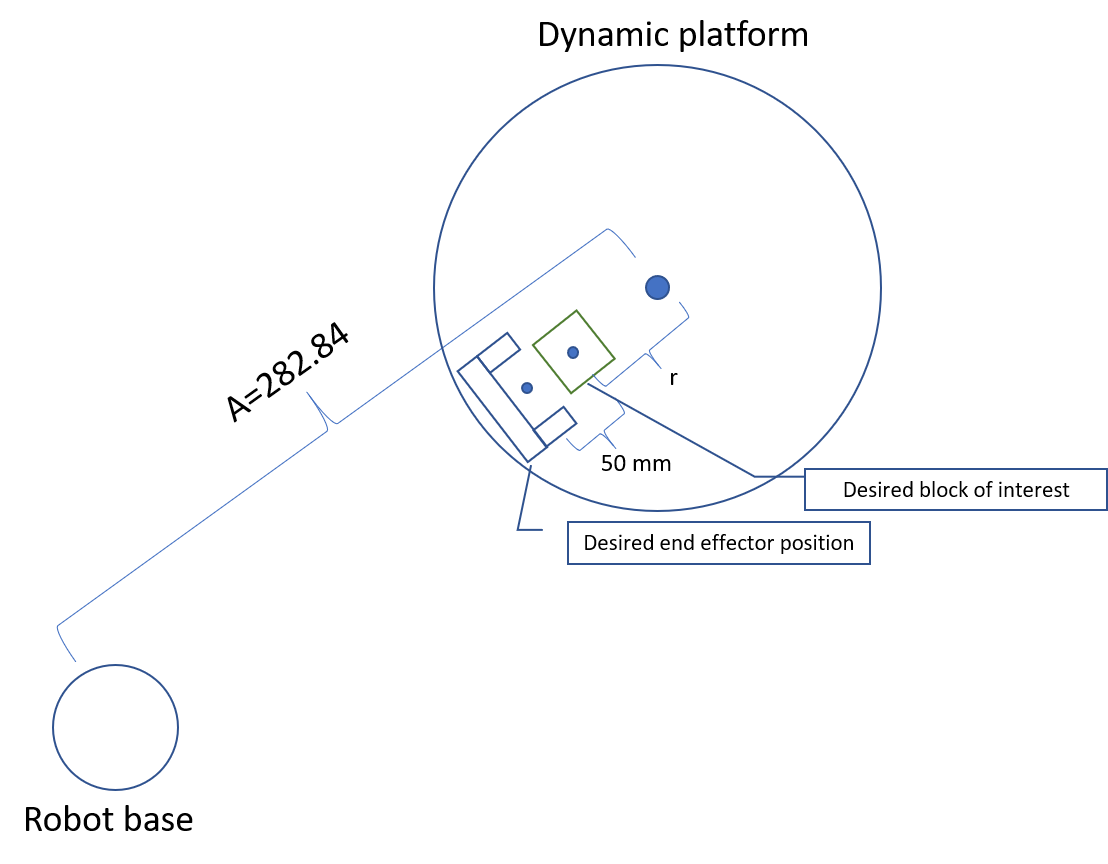
\includegraphics[width=0.7\textwidth]{Dynamic_block_representation.png}
\caption{Mathematically determining the end effector's position for a given block}
\label{dyn2}
\end{figure}
    
\begin{figure}[h]
\centering
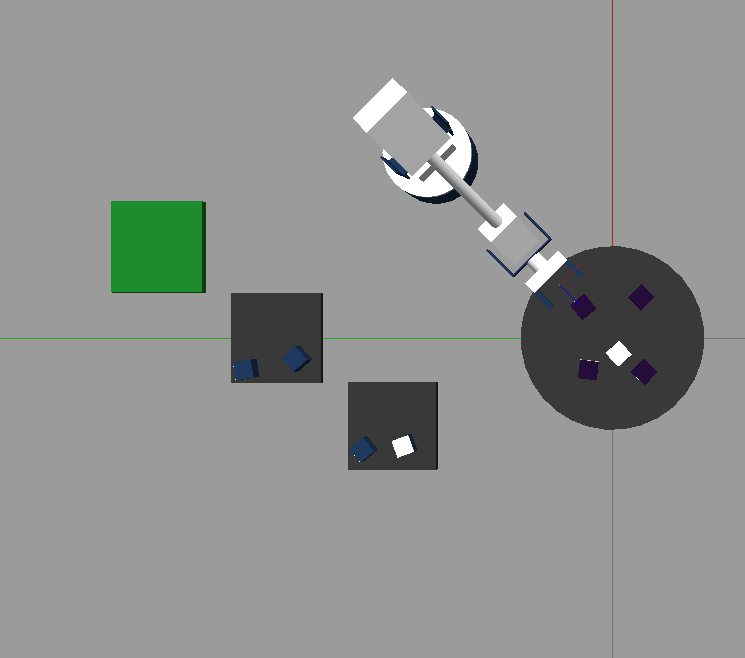
\includegraphics[width=0.7\textwidth]{Dynamic_pickup.png}
\caption{}
\label{dyn}
\end{figure}

\begin{figure}[h]
\centering
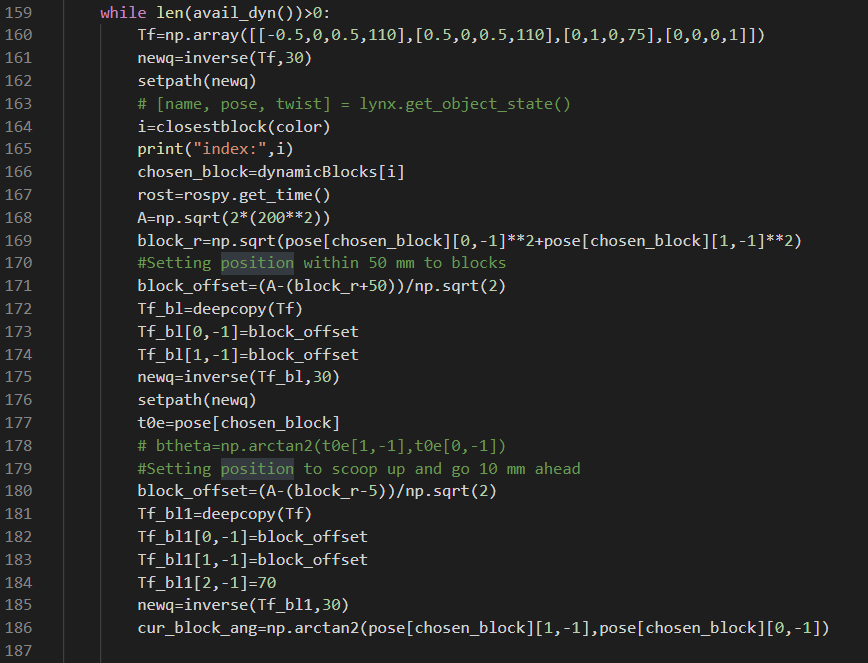
\includegraphics[width=0.7\textwidth]{dynamic_alg.png}
\caption{}
\label{dyn_alg}
\end{figure}

\begin{figure}[h]
\centering
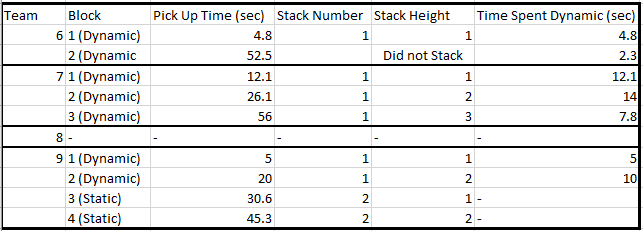
\includegraphics[width=0.8\textwidth]{Data_Competitions.png}
\caption{}
\label{data}
\end{figure}

\begin{figure}[h]
\centering
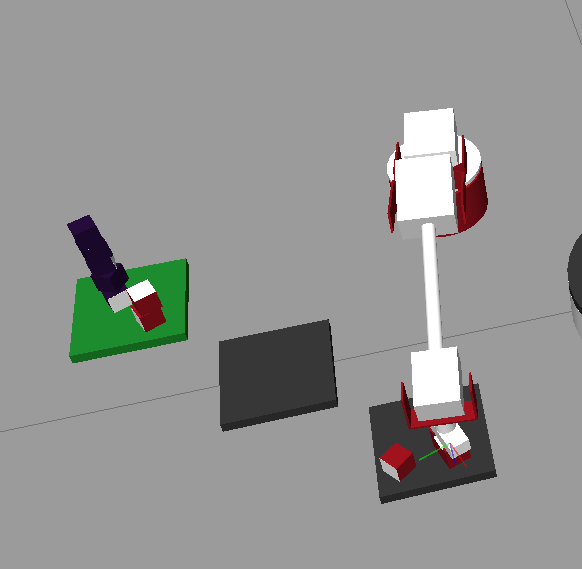
\includegraphics[width=0.5\textwidth]{IDEAL_STACK.png}
\caption{}
\label{ideal}
\end{figure}

\begin{figure}[h]
\centering
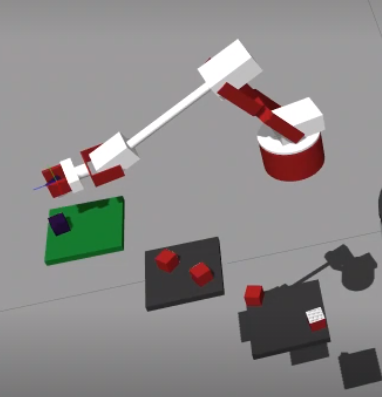
\includegraphics[width=0.5\textwidth]{Team_6_1Stack.png}
\caption{}
\label{t6}
\end{figure}

\begin{figure}[h]
\centering
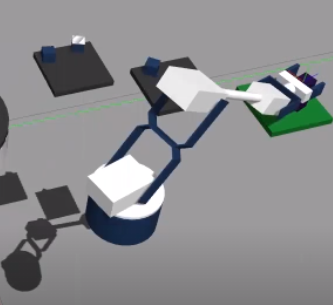
\includegraphics[width=0.6\textwidth]{Team_7_3Stack.png}
\caption{}
\label{t7}
\end{figure}

\begin{figure}[h]
\centering
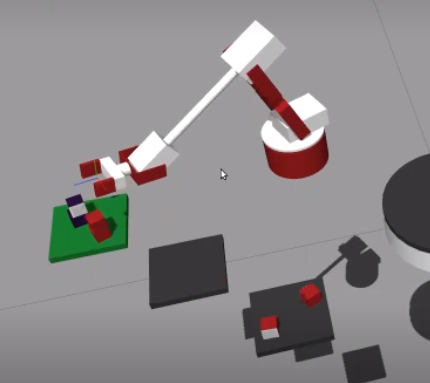
\includegraphics[width=0.6\textwidth]{Team_9_Stack.png}
\caption{}
\label{t9}
\end{figure}



\end{document}
